% Fronteirs template Version 2.4 Generated 2014/03/12 %%%
\documentclass{frontiersSCNS} % for Science articles

%\setcitestyle{square}
\usepackage{url,lineno}
\linenumbers

\copyrightyear{}
\pubyear{}

\def\journal{Genetics}%%% write here for which journal %%%
\def\DOI{} \def\articleType{Methods}
\def\keyFont{\fontsize{8}{11}\helveticabold }
\def\firstAuthorLast{Lawrence {et~al.}} %use et al only if is more than 1 author
\def\Authors{Travis J. Lawrence\,$^{1}$, Dana L. Carper\,$^{1}$, Kyle
  T. Kauffman\,$^{2}$, Katherine C.H. Amrine\,$^{1,3}$, Raymond S. Lee\,$^{4}$, Claudia
  J. Canales\,$^{4}$ and David H. Ardell\,$^{1,2*}$}
\def\Address{
$^{1}$Quantitative and Systems Biology, University of California, Merced, CA, USA \\
$^{2}$Molecular and Cell Biology Unit, University of California, Merced, CA, USA \\
$^{3}$Dept. of Viticulture and Enology, University of California, Davis, CA, USA \\
$^{4}$School of Engineering, University of California, Merced, CA, USA}
\def\corrAuthor{David H. Ardell}
\def\corrAddress{Molecular and Cell Biology, School of Natural Sciences, University of California, Merced, 5200 North Lake Road, Merced, CA , 95343, USA}
\def\corrEmail{dardell@ucmerced.edu}

\begin{document}
\onecolumn
\firstpage{1}

\title[FAST: Fast Analysis of Sequences Toolbox]{FAST: Fast Analysis of Sequences Toolbox}
\author[\firstAuthorLast ]{\Authors}
\address{}
\correspondance{}
\topic{}

\maketitle

\begin{abstract}
  FAST (Fast Analysis of Sequences Toolbox) provides a set of
  relatively simple yet powerful command-line tools to filter,
  transform, annotate and analyze biological sequence data. Modeled
  after the GNU (GNU's Not UNIX) Textutils such as {\tt grep}, {\tt
    cut}, and {\tt tr}, FAST tools such as {\tt fasgrep}, {\tt
    fascut}, and {\tt fastr} are designed for rapid prototyping of
  concise, production-scale reproducible bioinformatic workflows in a
  generic idiom with no programming required.  Interface consistency
  and conformity with GNU, Matlab, Perl, BioPerl, R and GenBank
  conventions are key to making FAST easy and rewarding to learn. FAST
  is also portable, easy to install, and secure, given its BioPerl and
  Perl foundations. The default data exchange format in FAST is
  MultiFastA (specifically, a restriction of BioPerl FastA format),
  while Sanger and Illumina 1.8+ FASTQ formatted files are also
  compatible.  FAST automates numerical, textual and taxonomic
  selection and filtering of sequence records, coordinate and
  annotation-based sequence extractions, and statistics including molecular biological
  statistics including composition and codon usage, and molecular
  population genetic statistics. FAST promotes reproducibility by
  reducing the need for manual data interventions and making it easier
  to document complex biological data processing. The command-line
  basis of FAST makes it easier to interactively investigate and
  control biological data at the speed of thought and brings the power
  of Perl and BioPerl to nonprogrammers. \tiny \keyFont{
  \section{Keywords:} Unix philosophy, MultiFASTA, pipeline,
  bioinformatic workflow, open source, BioPerl, regular expression,
  NCBI Taxonomy}
\end{abstract}

\section{Introduction}

Next Generation Sequencing (NGS) technology makes gigabyte- and
terabyte-scale biological sequence datasets commonplace.  Non-free
bioinformatic applications for basic sequence manipulation are often
monolithic with Graphical User Interfaces (GUIs)~\citep{Smith1994,
  Rampp2006, Librado01062009}.  Detailed documentation of
bioinformatic workflows, towards their ultimate reproducibility, often goes missing along scientific service chains

consistently and uniformly required for
publication. These trends fly in the face of calls for greater
reproducibility in modern biological research. Recent calls for
adequate documentation of bioinformatic and biostatistical workflows
and open source code sharing upon publication in bioinformatics
reproducible research and and biostatistics were motivated in part to
combat fraudulent research in
biomedicine~\citep{Peng01072009}. Open-source software in science
facilitates crowd-sourced verification, correction and extension of
code-based analysis~\citep{barnes2010publish}, and reuse of software
and data to make discoveries using public
data~\citep{Peng02122011}. The absence of adequate documentation for
analysis of high-dimensional data can obscure errors in processing
with profound potential ethical and financial
consequences~\citep{BaggerlyCoombes2009,hutson2010data,Baggerly01052011,Huang01072013}. In
one analysis, only 2 of eighteen published microarray gene-expression
analyses were completely reproducible in part because of proprietary
closed-source software~\citep{Ioannidis:2008cr}. Analytical errors are
a major source of retractions in the scientific
literature~\citep{Casadevall01092014}. Peer-review of scientific
software is generally not yet required for publication but seen as
necessary for integrity of the scientific enterprise across fields and
requiring more computational training for all
scientists~\citep{Morin13042012,Joppa17052013}. Publication and
documentation of bioinformatics workflows simplifies post-publication
validation of research findings and may help reduce the temptation to
fish for significance and encourage more objectivity in data analysis
and interpretation~\citep{Boulesteix01022010}

To reduce human error and increase reproducibility in the management
and documentable processing of biological data, it is desirable to
create self-documenting automated bioinformatic workflows --- scripts
and other literate programming that encode scientific workflows for
machine processing of biological data. Web-based open-source workflow
suites such as Galaxy~\citep{galaxy14}, Taverna~\citep{CPE:CPE993} and
BioExtract~\citep{Lushbough01072011} facilitate this, but an even more
rapid and time-tested development platform for rapid prototyping of reproducible
workflows is the UNIX command-line, specifically UNIX pipelines.

The FAST utilities are modeled after the standard Unix
toolkit\citep{Peek2001} and follow the Unix philosophy to ``do one
thing and do it well'' \citep{Stutz2000}.


Command-line utilities for bioinformatics such as the EMBOSS
package~\citep{Rice2000} or the scripts that come with
BioPerl~\citep{Stajich2002} typically offer suites of tools with
simple, well-defined functions that lend themselves to scripting, but
are not necessarily designed according to the UNIX toolbox philosophy specifically to interoperate through
composition.

 They are written in Perl
using BioPerl packages \citep{Stajich2002}. This makes FAST utilities
easy to adopt if you are familiar with the Unix toolbox and allows
fast sequence analysis even on large datasets. Extensive
documentation has been developed for each utility along with useful
error messages following the recommendations of \citep{Seemann2013} to
increase usability. Lastly, FAST is open source, which makes it
available to anyone free of cost. This is in line with the call to
make science more assessable, open, and reproducible by other
scientists and the public \citep{Groves2012}.

\section{Design}

An overview of Version 1.0 of the FAST project is shown in
Figure~\ref{fig:01}. Descriptions of the function of utilities along
with GNU Textutil analogs are given in Table~\ref{tab:01}.

\begin{table}[!t]
\textbf{\refstepcounter{table}\label{tab:01} Table \arabic{table}.}{
  FAST 1.0 utilities }

\processtable{ }
{\begin{tabular}{llll}\toprule
    Tool  & Function  & Textutil analog & Default field processed  \\\midrule
    {\tt fasgrep} & regex selection of records & {\tt grep} & identifiers\\
    {\tt fasfilter} & numerical selection of records &  & identifiers \\
    {\tt fastax} & taxonomic selection of records &  & descriptions \\
    {\tt fashead} & order-based selection of records & {\tt head} & \\
    {\tt fastail} & order-based selection of records &  {\tt tail}  &  \\
    {\tt fascut} & index-based selection and reordering of data  &  {\tt cut}  & sequences \\
    {\tt fasuniq} &  record reduction by content and order & {\tt uniq} & sequences \\
    {\tt alncut} & selection of sites by content &  & sequences \\
    {\tt gbfalncut} & selection of sites by features &  & sequences \\
    {\tt fassort} & numerical or text sorting of records  & {\tt sort} & identifiers\\
    {\tt fastaxsort} & taxonomic sorting of records &  & identifiers \\
    {\tt faspaste} & merging of records &  {\tt paste} & sequences \\
    {\tt fastr} & character transformations on records & {\tt tr} & identifiers\\
    {\tt fassub} & regex substitutions on records &  & identifiers \\
    {\tt faslen} & annotate sequence lengths &  & descriptions \\
    {\tt fascomp} & annotate monomeric compositions &  & descriptions \\
    {\tt fascodon} & annotate codon usage &  & descriptions \\
    {\tt fasxl} & annotate biological translations &  & descriptions \\
    {\tt fasrc} & annotate reverse complements &  & descriptions \\
    {\tt fasconvert} & convert format of records &  &  \\
    {\tt gbfgrep} & select feature neighborhoods by context & {\tt grep}  & features \\
    {\tt gbf2fas} & emit sequences by regex matching on features  & {\tt grep}  & features\\
    {\tt alnpi} & molecular population genetic statistics &  &  \\
    {\tt faswc} & tally sequences and characters & {\tt wc} & sequences \\
\end{tabular}}{}
\end{table}

FAST is split into three categories selection, transformation, and
annotation and analysis. The selection category contains utilities
designed to select sequences and sites from alignments based on
several different criteria. For example fasgrep selects sequences by
matching a regular expression to the ID, description, or sequence. The
transformation utilities are used to modify the ID, description,
sequence, or order of sequences using several criteria. For example,
fastaxsort sorts sequences within a multifasta file based on NCBI
taxonomy \citep{Benson2009, Sayers2009}. The annotation and analysis
category contains utilities to calculate sequence composition, codon
usage, sequence length, and basic population genetic
statistics. Additionally these utilities can also append the results
of the analysis to the sequence description, which then can be used as
selection and sorting criteria by the utilities in the selection
category.

Learnability of the FAST tools is helped by making interface
components such as specific options, consistent with the standard UNIX
tools and across the FAST suite. Learning one FAST tool generally
helps the user anticipate how to use others. In addition,
specification of numerical ranges, regular expressions and other
useful parameters follows standard Perl and UNIX conventions, all with
the intent of making the tools fast and easy to learn.

\section{Implementation Details and Benchmarking}

All FAST utilities can process files or input on what is called the
``standard input'' stream. They all by default out to the ``standard
output'' stream which may be connected to the ``standard input'' of
another utility by a UNIX ``pipe.'' It is this latter facility that
eases serial processing of data. Since most FAST utilities process
sequences inline, they should mostly linear runtime complexity in
number of sequences. Two exceptions to inline processing in FAST
utilities concern {\tt fassort } and {\tt fastail} which both require
some paging of data into temporrary files. However, some preliminary
benchmarking suggests that {\tt fassort} runtimes also scale linearly in
sequence number (fig~\ref{fig:02}). Benchmarking was performed using
the Benchmark v1.15 perl module on a MacBook Pro ??Ghz Intel
i7, 8 Gb of RAM. The average CPU time of 100 iterations to complete
the analysis of six datasets consisting of 25,000, 250,000, or
1,000,000 100bp sequences (fig 2A) and 10,000, 100,000, or 1,000,000 1,000bp sequences (fig 2B) were used to estimate performance.  

FAST is compatible with the zero-based indexing if the sequence
identifier is thought as the zero$^{th}$ field of the identifier
line. This field must exist in Data selection in FAST is
one-based as is conventional BioPerl coordinates and bioinformatics
generally.

FAST supports automated logging to ease the reproducibility of
workflows. The BioPerl backend of FAST was version 1.6.901 downloaded in January,
2012. BioPerl dependencies of FAST scripts were analyzed with the Cava
packager (\url{http://www.cavapackager.com}). To fix some problems with
I/O, the SeqIO components were updated to version 1.6.923 on
June 4, 2014 and the Root components were updated on July 10, 2014 (github commit 50f87e9a4d). 
Some customizations of the BioPerl code-base were introduced, primarily 
to enable the translation of sequences containing gaps. 

\section{Installation and Usage Examples}

\subsection{Installation and Dependencies}
FAST requires a working Perl installation and is distributed through
the Comprehensive Perl Archive Network (CPAN). In a manual install,
after download, installation follows standard Perl install procedure:
{\tt perl Makefile.PL; make; make test; (sudo) make install}. A small
footprint of BioPerl dependencies has been packaged together in the
FAST namespace. Other CPAN dependencies can be detected and installed
by the {\tt cpan} package manager. A fully automated install may on
many systems be initiated by executing {\tt perl -MCPAN -e 'install
  FAST'}.

\subsection{Selecting sequences by encoded motifs }

An advantage of the annotation approach in FAST is the ability to
select and sort sequences by attributes computed and annotated into
data by utilities upstream in the pipeline. For example, to select
protein-coding genes from a file {\tt cds.fas} whose translations
contain the {\it N}-glycosylation amino acid
motif~\citep{KornfieldKornfield85}, one could execute:

\begin{verbatim}
fasxl -a cds.fas | fasgrep -t xl0 "N[^P][ST][^P]" | fascut -f 1..-2
\end{verbatim}
 
The first command in the pipeline translates each sequence and appends
the translation to the description with the tag ``xl0'' (indicating
translation in the zeroth reading frame). The second command in the
pipeline does a regex match using the specified motif pattern on the
value of a ``name:value'' pair in the description with tag ``xl0'',
hence processing the annotations produced by {\tt fasxl}. The regex
argument to {\tt fasgrep} is quoted to protect the argument from
interpretation by the shell. The last command in the pipeline removes
the last field in the description, restoring records as they were
before they were annotated by {\tt fasxl}.

\subsection{Sorting sequences by third codon position composition}

Another example illustrates the powerful expression of ranges in {\tt
  fascut}. An optional ``by'' parameter in ranges allows increments or
decrements in steps larger than one. To extract the third codon
position bases from a gene, annotate their compositions, and sort
sequences by their third-position adenosine contents, do:

\begin{verbatim}
fascut 1:-1:3 cds.fas | fascomp | fassort -nt comp_A
\end{verbatim}

\section{Concluding Remarks}

Planned additions in future versions of FAST include {\tt fasrand} and
{\tt alnrand} for sampling, permutations and bootstrapping of
sequences and sites, respectively.

\section*{Availability}

FAST is available through the Comprehensive Perl Archive Network
(CPAN) at \url{http://search.cpan.org/~dhard/FAST}

\section*{Disclosure/Conflict-of-Interest Statement}

The authors declare that the research was conducted in the absence of
any commercial or financial relationships that could be construed as a
potential conflict of interest.

\section*{Author Contributions}

D.H.A. conceived, designed, and wrote much of FAST. T.J.L. contributed
major code factorizations and reorganization and {\tt
  fastail}. K.T.K. contributed code including {\tt faspaste}, and {\tt
  fashead}. R.S.L. contributed an analysis of code dependencies for
the FAST installer. All authors, especially D.L.C. and C.J.C.,
contributed documentation, testing, and code fixes. K.C.H.A. and
D.H.A. wrote the FAST Cookbook. D.H.A. wrote the paper with major
contributions from D.L.C. and T.J.L. All authors made minor
contributions to the manuscript, reviewed the final version of the
manuscript and agree to be accountable for its contents.

\section*{Acknowledgement}
We acknowledge Christopher Clark for help in establishing a git
repository for FAST. D.H.A. gratefully acknowledges Professors Laura
Landweber, Siv Andersson and Leif Kirsebom in whose laboratories the
FAST tools were first developed as well as the Linnaeus Centre for
Bioinformatics at Uppsala University.

\paragraph{Funding\textcolon} D.H.A. gratefully acknowledges an NSF-DBI
Postdoctoral Fellowship in Biological Informatics and awards to
D.H.A. from UC Merced's Graduate Research Council and a Chancellor's
Award from UC Merced's second Chancellor Sung-Mo Kang.

\bibliographystyle{frontiersinSCNS&ENG} % for Science and Engineering articles
\bibliography{FAST}

\section*{Figures}

\begin{figure}
\begin{center}
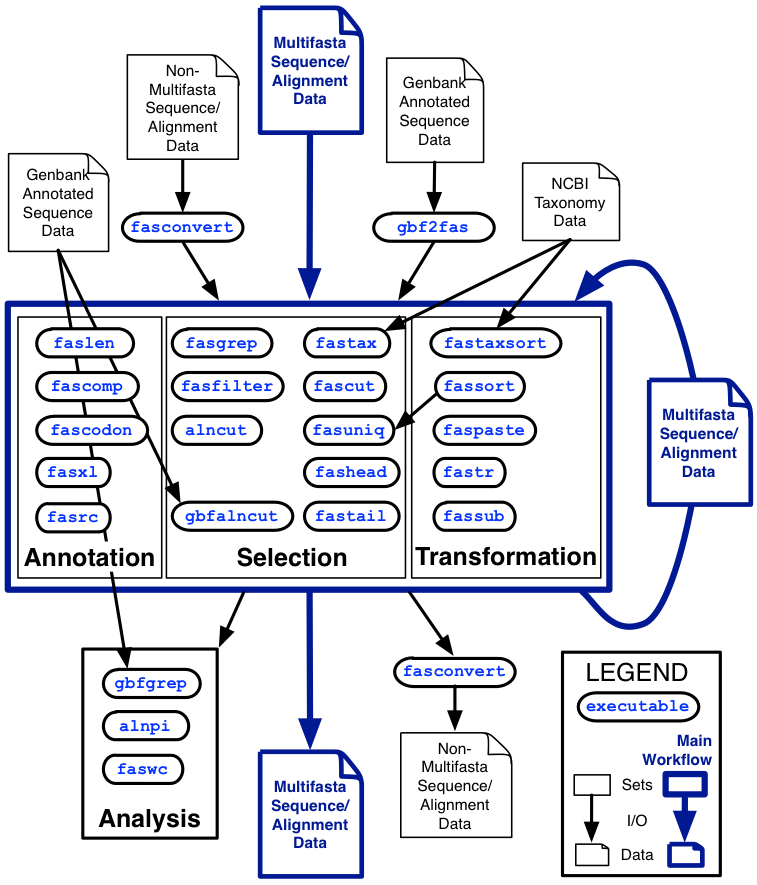
\includegraphics[width=4.5in]{FAST_v7}% This is a *.jpg file
\end{center}
 \textbf{\refstepcounter{figure}\label{fig:01} Figure
   \arabic{figure}.}{ FAST version 1.0 with data and workflow
   dependencies indicated.}
\end{figure}

\begin{figure}
\begin{center}
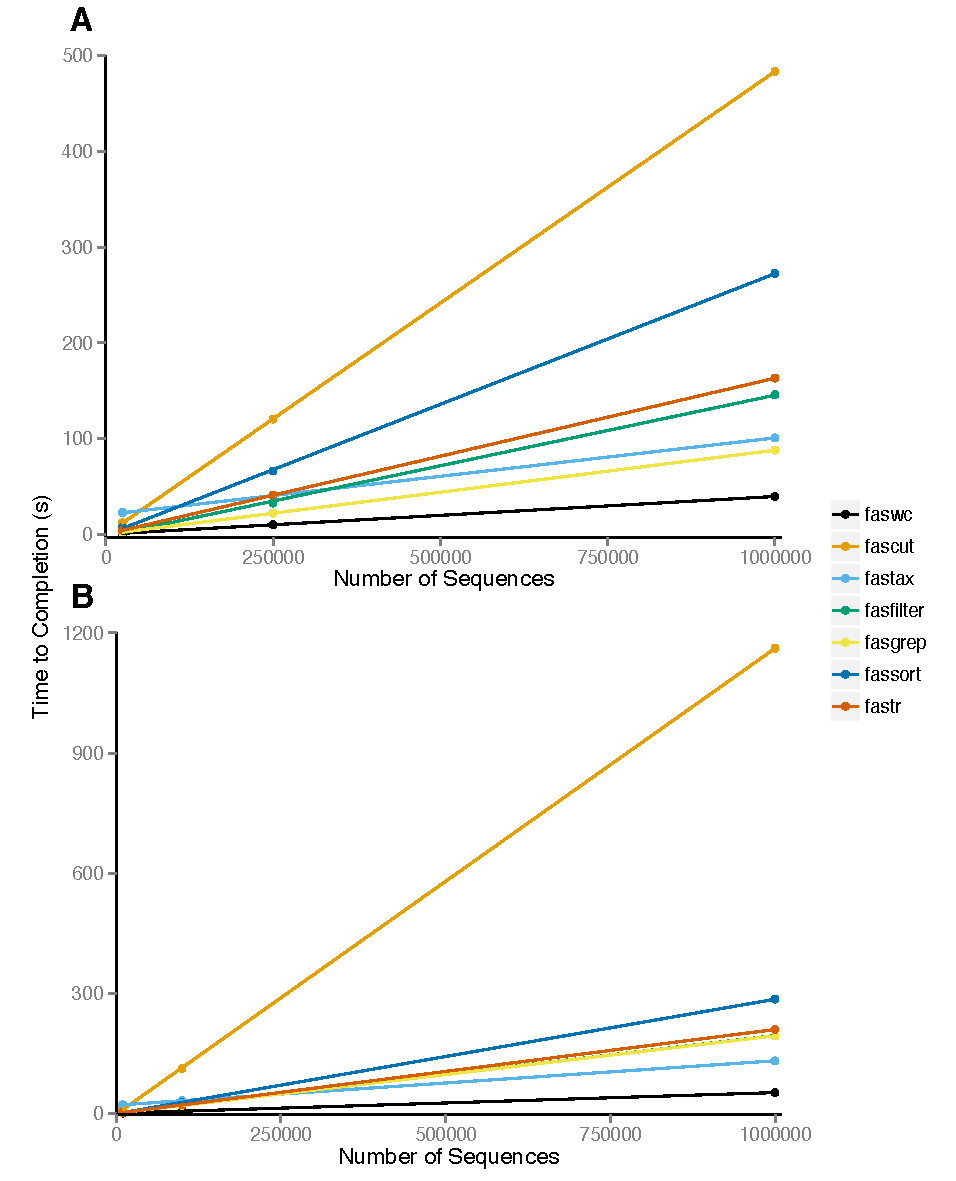
\includegraphics{Figure2}
\end{center}
\textbf{\refstepcounter{figure}\label{fig:02} Figure
  \arabic{figure}.}{ Average processor time of 100 repetitions
  required to complete analysis using indicated utility. Utilities
  were run on six datasets consisting of (a) 25000, 250000, and
  1000000 100bp sequences and (b) 10000, 100000, and 1000000 1000bp
  sequences. }
\end{figure}


\end{document}
